\documentclass[crop,tikz]{standalone}
\usepackage{tikz}

\tikzstyle{Node}=[draw,rounded rectangle]
\tikzstyle{Line}=[-stealth, thick]
\tikzstyle{Red}=[fill=red!20]
\tikzstyle{Green}=[fill=green!20]
\tikzstyle{Blue}=[fill=blue!20]
\tikzstyle{Orange}=[fill=orange!20]

\usetikzlibrary{shapes.misc}

\begin{document}

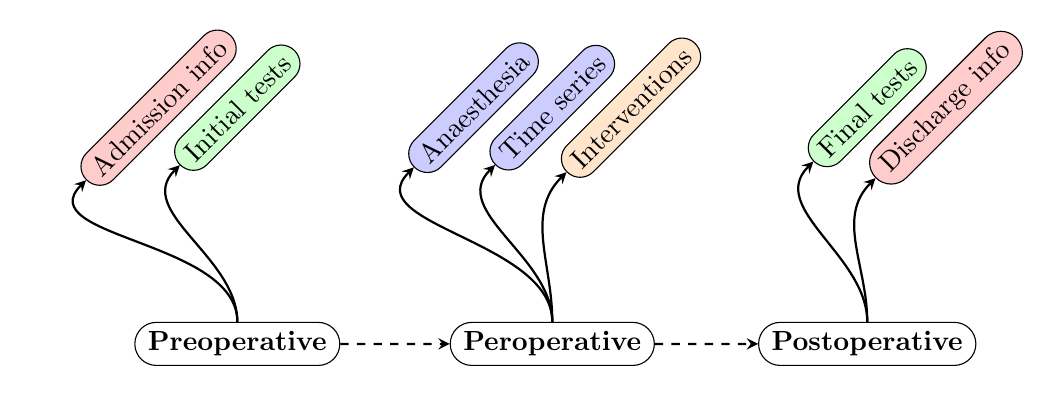
\begin{tikzpicture}

    \node[Node] (pre) at (0, 0) {\textbf{Preoperative}};
    \node[Node] (per) at (4, 0) {\textbf{Peroperative}};
    \node[Node] (pos) at (8, 0) {\textbf{Postoperative}};
    
    \node[Node,rotate=45,Red] (adm) at (-1, 3) {Admission info};
    \node[Node,rotate=45,Green] (ini) at (0, 3) {Initial tests};
    
    \node[Node,rotate=45,Blue] (ana) at (3, 3) {Anaesthesia};
    \node[Node,rotate=45,Blue] (tim) at (4, 3) {Time series};
    \node[Node,rotate=45,Orange] (int) at (5, 3) {Interventions};
    
    \node[Node,rotate=45,Green] (lat) at (8, 3) {Final tests};
    \node[Node,rotate=45,Red] (dis) at (9, 3) {Discharge info};

    \draw[Line,dashed] (pre) to (per);
    \draw[Line,dashed] (per) to (pos);

    \draw[Line] (pre) to[out=90, in=225] (adm.west);
    \draw[Line] (pre) to[out=90, in=225] (ini.west);
    
    \draw[Line] (per) to[out=90, in=225] (ana.west);
    \draw[Line] (per) to[out=90, in=225] (tim.west);
    \draw[Line] (per) to[out=90, in=225] (int.west);
    
    \draw[Line] (pos) to[out=90, in=225] (lat.west);
    \draw[Line] (pos) to[out=90, in=225] (dis.west);

\end{tikzpicture}

\end{document}
